\title{Machine Learning \\ \bigskip WS2010/11\\ \bigskip Exercise 2}
\author{
        Benjamin Bachhuber \\
                (1028430)\\
                \and
        Patrick Marschik\\
        (0625039)
}
\date{\today}

\documentclass[a4paper,12pt]{article}
\usepackage{verbatim}
\usepackage{graphicx}
\usepackage{color}
\usepackage{array}
\usepackage{xspace}
\usepackage{acronym}
\usepackage{rotating}

\definecolor{LinkColor}{rgb}{0,0,0.7}

\usepackage[
bookmarks=true, % PDF bookmarks allowed. NB! The level depth of bookmarks is the same as in the TOC.
unicode=true, % PDF bookmarks in Unicode.
bookmarksnumbered=true, % Section numbers in PDF bookmarks.
bookmarksopenlevel=1, % The open level in PDF bookmarks.
hyperindex=true, % Hyperlinked index.
plainpages=false, % Name arabic and roman page numbers differently.
colorlinks=true, % Links are marked as coloured text, not coloured box.
linkcolor=linkc, % The colour for in-document links (e.g. in the table of contents).
citecolor = citec, % The colour for bibliographic citations.
urlcolor=urlc, % The colour for hyperlinks to the Net.
pdfpagelayout=OneColumn % Continuous page scrolling.
]{hyperref}
\hypersetup{
  colorlinks=true,
  linkcolor=LinkColor,
  citecolor=LinkColor,
  filecolor=LinkColor,
  menucolor=LinkColor,
  pagecolor=LinkColor,
  urlcolor=LinkColor
}

\usepackage{amsmath}
\usepackage{amsthm}
\usepackage{amsfonts}

\usepackage{tocloft}

\newcommand{\dss}{soybean-small\xspace}
\newcommand{\dsn}{nursery\xspace}
\newcommand{\dsa}{arrhythmia\xspace}
\newcommand{\linsearch}{LinearNNSearch\xspace}

\acrodef{WEKA}{Waikato Environment for Knowledge Analysis}

\begin{document}
\maketitle

\newcommand{\fittable}[1]{\begin{center}
\resizebox{\textwidth}{!}{#1}\end{center}
}

\newcommand{\img}[4]{
 \begin{figure}[!htp]
\centering
  \includegraphics[width=#1\textwidth]{#2}
  \caption{\emph{#3}}
  \label{#4}
 \end{figure}
}
\newcommand{\imgit}[4]{
\\[\intextsep]
\begin{minipage}{\linewidth}
  \centering%
  \includegraphics[width=#1\textwidth,clip=]{#2}%
  \figcaption{\emph{#3}}%
  \label{#4}%
\end{minipage}
\\[\intextsep]
}

\newcommand{\imgitX}[2]{
  {\centering
\fbox{
\begin{minipage}{#1\textwidth}
  \vskip .5em
  \centering
  \includegraphics[width=#1\textwidth]{#2}
  \vskip .5em
\end{minipage}
}
  }
}


\newpage

\tableofcontents

\section{Introduction}

The prisoner's dilemma is one of the fundamental problems in game theory.\\
In the prisoners dilemma there are two prisoner's.
Each of them has to decide whether to cooperate with an opponent, or defect.
Both prisoners make a choice and then their decisions are revealed. 

They receive a payoff according to the following table: 

\begin{table*}[h]
	\centering
		\begin{tabular}{| l | r | r |}
		\hline
			Action of A / Action of B & Comply & Defect \\
			Comply                    & 3 / 3 & 5 / 0\\
			Defect                    & 0 / 5 & 1 / 1\\
			\hline
		\end{tabular}  
\end{table*}

Since the strategies for a game with one turn or with a deterministic amount of games is fairly predictable,
the so called \textit{Iterate Prisoner's Dilemma} was used.
In this special kind of Prisoner's Dilemma none of the prisoner's knows how many rounds are played.

\section{Technical Description}

One of the most important decisions is which agents are needed and what their main tasks are.
The following use case diagramm helped was very useful in this process of decision making:

The use case diagram shows (see fig. \ref{fig:usecase} on page \pageref{fig:usecase}) that two agent classes are needed:
\texttt{PrisonerAgent} (see fig. \ref{fig:state_prisoner} on page \pageref{fig:state_prisoner}) and \texttt{GamemasterAgent} (see fig. \ref{fig:state_gm} on page \pageref{fig:state_gm}).

The agents required to communicate with each other on several channels.
There are different forms of communication which are required:

\begin{itemize}
	\item The \texttt{GamemasterAgent} has to be able to ask the the PrisonerAgents if they are guilty.
	\item The \texttt{PrisonerAgent}s has to be able to answer if they are guilty.
	\item A \texttt{PrisonerAgent} has to be able to receive notifications about the game state from the \texttt{GamemasterAgent}.
	\item The \texttt{GamemasterAgent} has to be able to inform the \texttt{PrisonerAgent}s
		-- that requested notifications about changes -- about the current game state.
\end{itemize}

These tasks basically require two different interaction protocols (see fig. \ref{fig:sequence} on \pageref{fig:sequence} on how they work together.)

\begin{description}
	\item[ArchieveREInitiator \& ArchieveREResponder]\hfill \\
	 	This protocol is used to to enable the Agents to ask and answer the question of guiltiness.
		Furthermore the special case of the FIPA-query protocol was used.
		This protocol queries an agent about what he believes about a certain state -- in our case it's guiltyness.
	\item[SubscriptionInitiator \& SubscriptionResponder] \hfill \\
		Enables the \texttt{PrisonerAgent}s to register at the \texttt{GamemasterAgent} receive notification.
		The \texttt{GamemasterAgent} in turn sends the results of the round -- i.e. what each agent voted -- to all it's subscribers.
\end{description}


\section{Conclusion}
The prisoner's dilemma is a good example to show the strength and weaknesses of Multi Agent Systems.
Using Multi Agent Systems for small projects seems like an overhead.
In in large projects however Multi Agents System are a powerful architecture.

\newpage

\appendix

\section{Diagrams}

\begin{figure}[h]
	\centering
	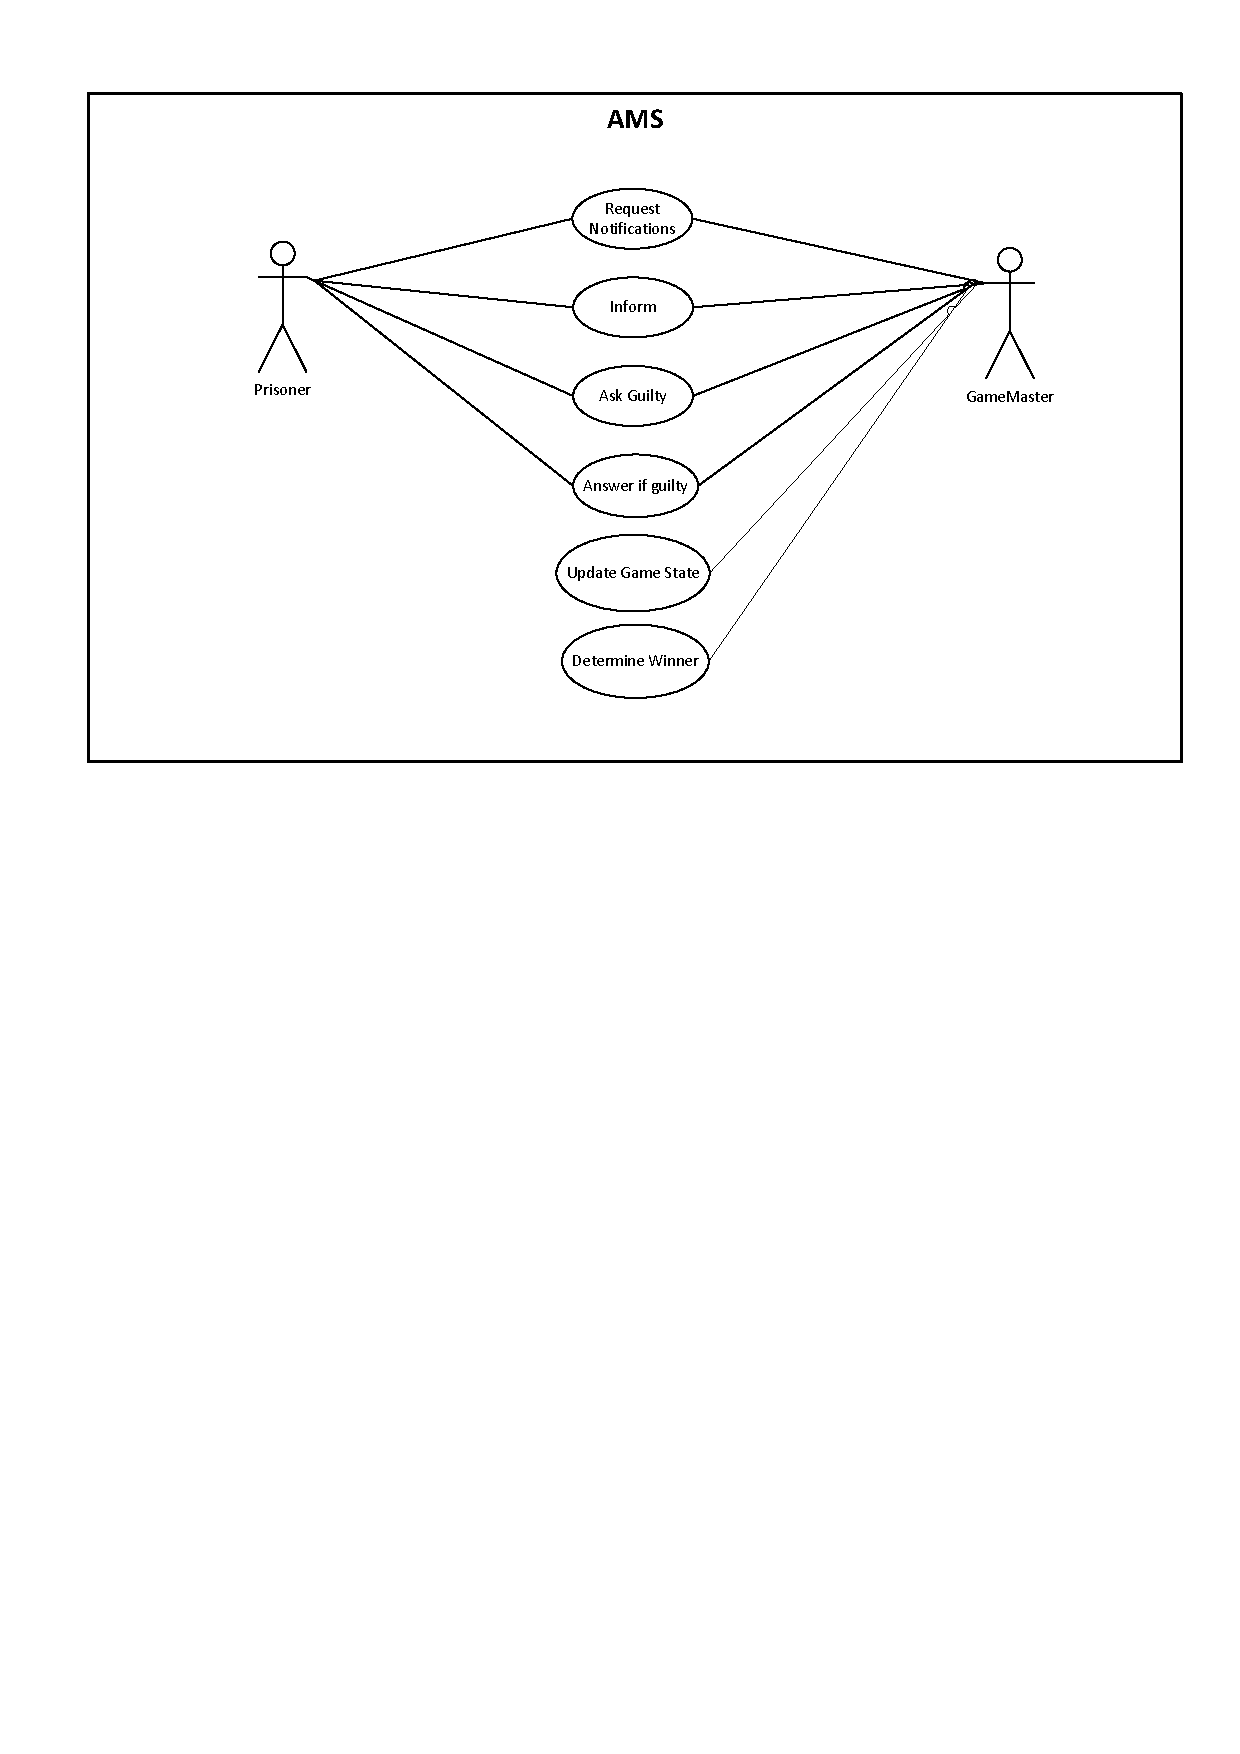
\includegraphics[width=400px]{usecases.pdf}
	\caption{Use-Case diagram}
	\label{fig:usecase}
\end{figure}

\begin{figure}[h]
	\centering
	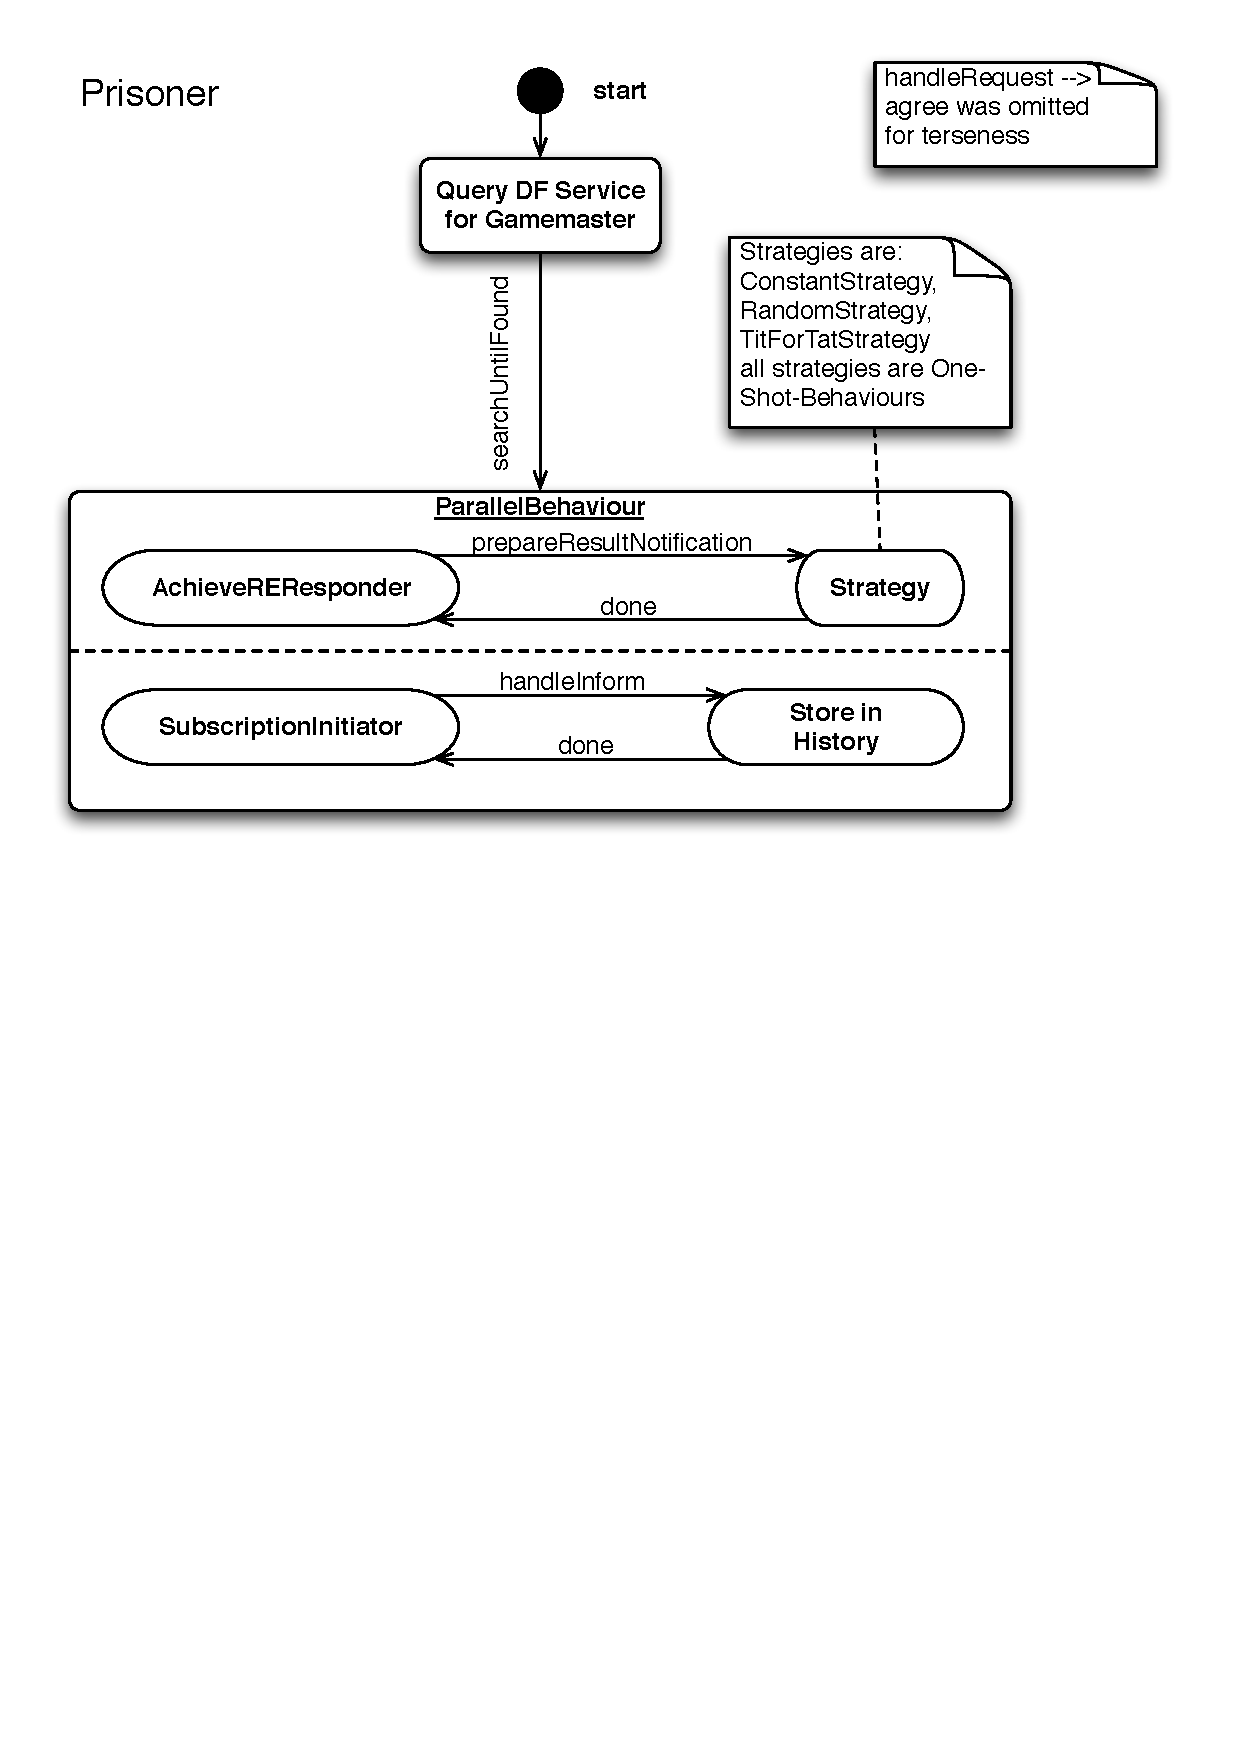
\includegraphics[width=400px]{chart1_Part2.pdf}
	\caption{State diagram for \texttt{PrisonerAgent}}
	\label{fig:state_prisoner}
\end{figure}

\begin{figure}[h]
	\centering
	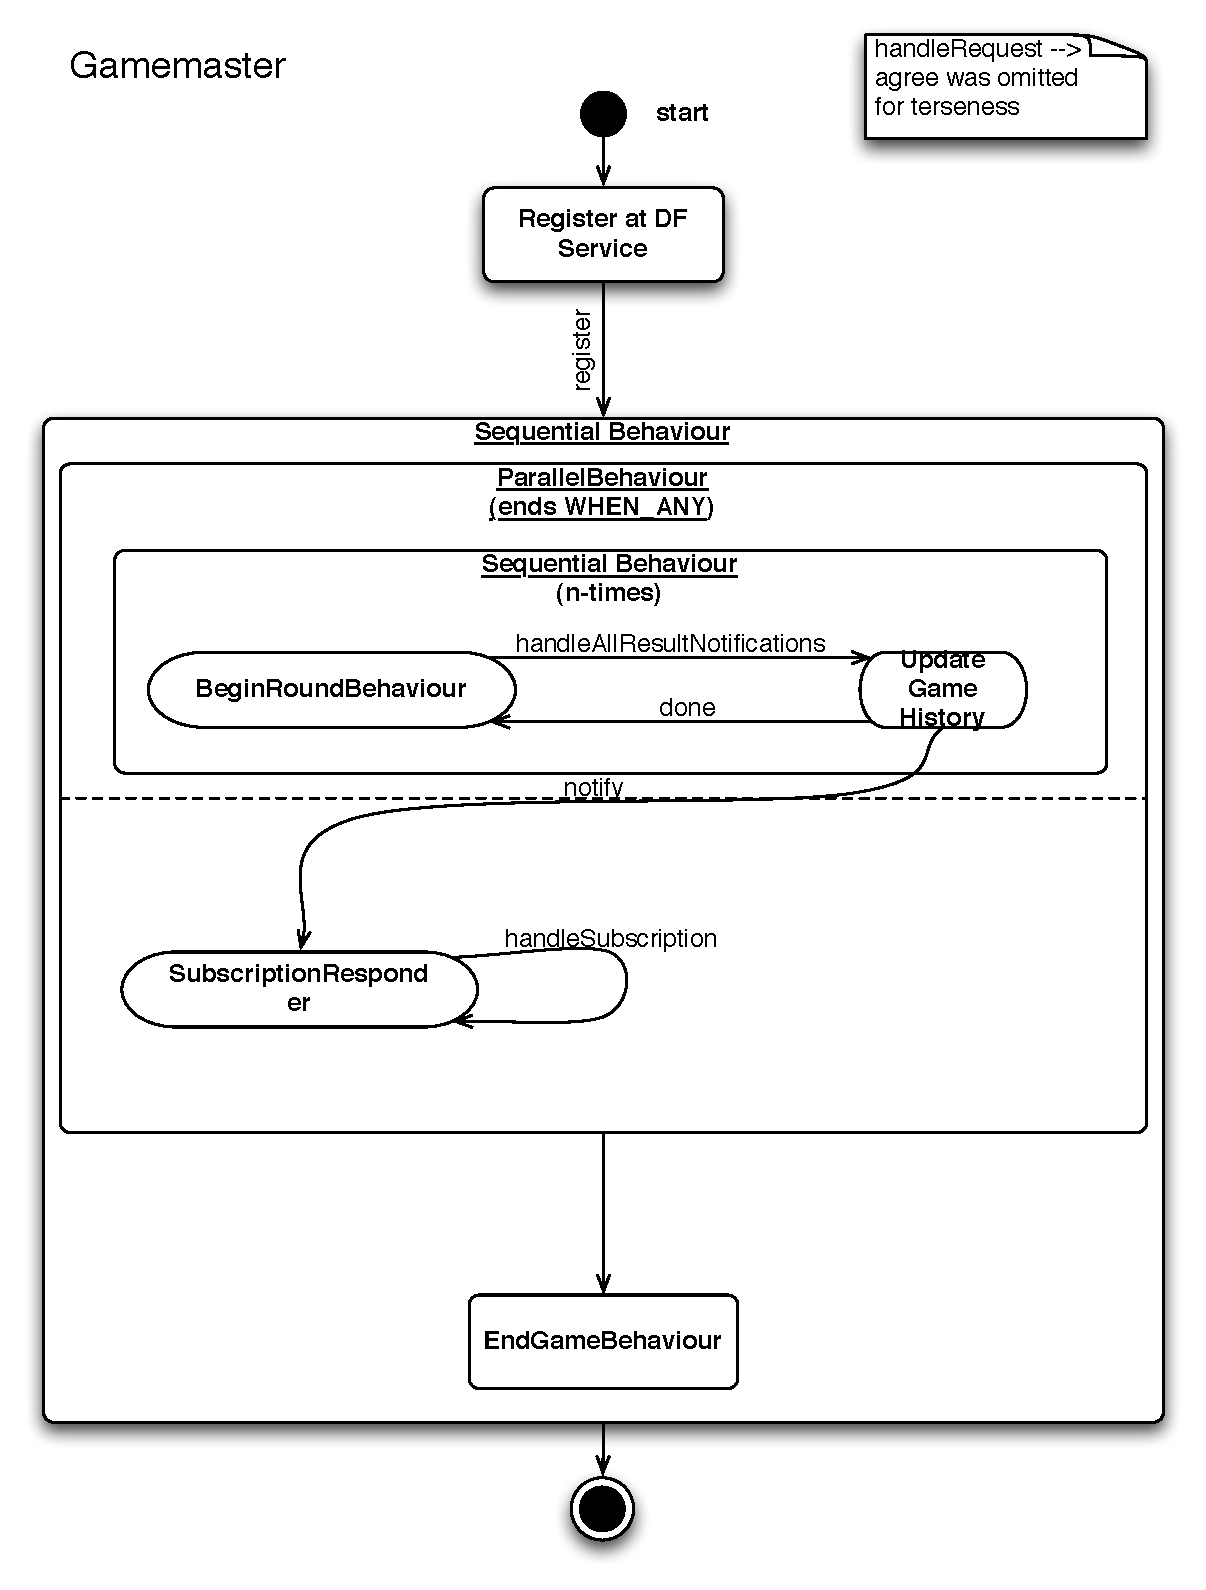
\includegraphics[width=400px]{chart1_Part3.pdf}
	\caption{State diagram for \texttt{GamemasterAgent}}
	\label{fig:state_gm}
\end{figure}

\begin{figure}[h]
	\centering
	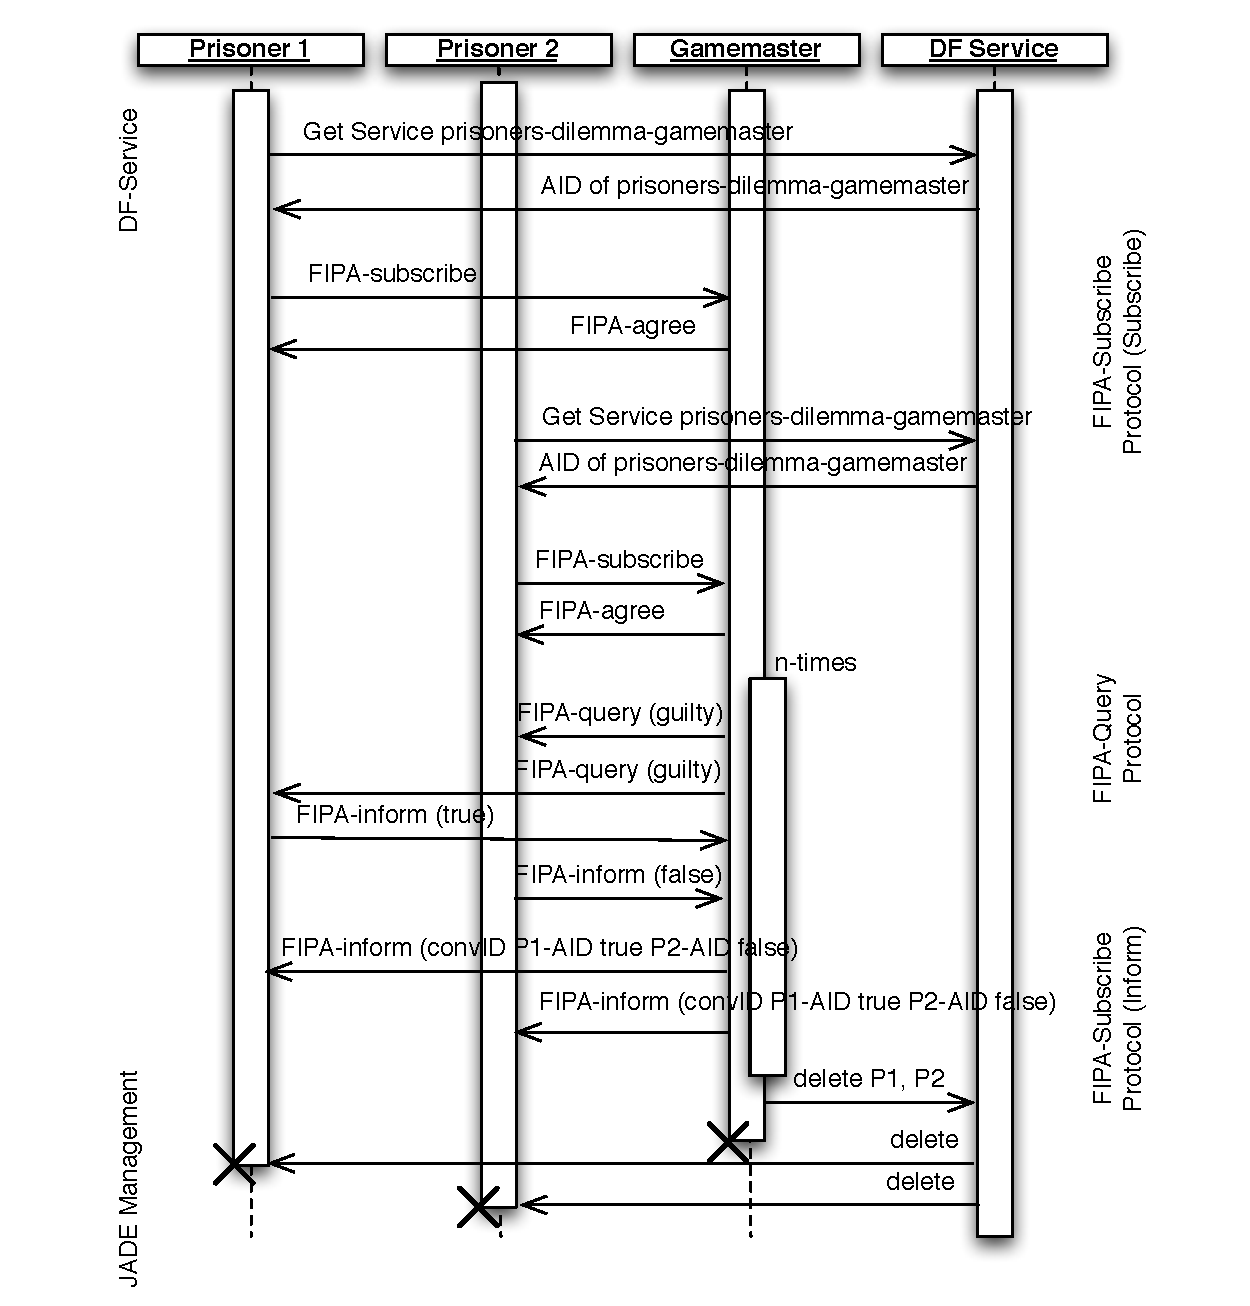
\includegraphics[width=400px]{chart1_Part1.pdf}
	\caption{Sequence diagram}
	\label{fig:sequence}
\end{figure}

%#\bibliographystyle{abbrv}
%#\bibliography{main}

\end{document}
This is never printed

